\chapter{Stima del modello del sistema}\label{cap:stimaModello}

\begin{minipage}{12cm}\textit{
	In questo capitolo viene affrontato il problema della stima dei parametri del modello reale, in un equivalente lineare matematico, necessario per le simulazioni future e validare i risultati matematici precedenti.}
\end{minipage}

\vspace*{1cm}
\noindent
Partendo dall'esperimento con l'\nameref{lst:ondaTrapezoidale} per eccitare il sistema senza raggiungere la saturazione della tensione $ V_2 $ (ricordiamo che in uscita abbiamo un derivatore filtrato, quindi ogni onda quadra genera automaticamente una forte derivata), si è puntato a ricavare un modello lineare prima della corrente in $ I_T $ e successivamente della tensione $ V_2 $.\\
Essendo il driver di corrente intrinsecamente non lineare, specie nei pressi della Dead-zone, il cui taglio si è visto non essere netto come si spererebbe, si è cercato di ottenere un buon fitting nei transitori del sistema, dove la dinamica è più lineare e "pulita".\\
Questa stima è ovviamente qualitativa e permette di dimensionare tempi di risposta e sistemi di controllo, le non linearità presenti hanno però dinamiche molto rapide, e grazie a questa proprietà, il controllo pensato lineare che vedremo in seguito, continua ad essere valido anche nel caso reale.
Il modello stimato è $ P_{pos} $ (eq \ref{eq:FuncTrasfTotPos}), per rendere più intuitivi i risultati.

\newpage

\section{Metodo Di stima automatico}
Il metodo di stima automatico passa per l'uso del \cite*{IdentificationToolbox} di Matlab, ed è usato allo scopo di ottenere una funzione di trasferimento SISO tra l'ingresso del duty-cycle (PWM) e la tensione sul secondario V2. Avendo a disposizione anche i dati della corrente sul primario, anche se poco sensibili, si è deciso di dividere la stima in 2 fasi: prima si è stimato il modello della corrente nel primario, e a causa della sua scarsa sensibilità di misura (risultato \ref{result:Istep}) si è usato il segnale ricostruito come ingresso per la stima della dinamica della tensione sul secondario.\\
Il numero di \textit{Poli} e \textit{Zeri} di entrambe le funzioni di trasferimento sono state scelte partendo dall'analisi teorica descritta nella sezione \nameref{subsec:ModelloFisico}, e il codice è presente in appendice a \nameref{lst:autoEst}.

\begin{table}[H]
	\centering
	\caption[Stime parametri con \cite*{IdentificationToolbox}]{Stime parametri con \cite*{IdentificationToolbox}}		\label{tab:stimaAutomaticaParametri}
	\vspace{1mm}
	\begin{tabular}[t]{||l|c|c||}
		\hline
		\multicolumn{1}{||c}{\textbf{Funzione}}            & \multicolumn{1}{|c}{\textbf{Input}} & \multicolumn{1}{|c||}{\textbf{Input}} \\
		\hline\hline
		                                                   &                                     &                                       \\[-3mm]
		$\hat{P}_{p_{wm} I_1}(s) = \frac{970}{s+110}$      & PWM                                 & $I_1$                                 \\[3mm]

		$\hat{P}_{I_1 V_2}(s) = -\frac{0.44\,s+11}{s+200}$ & $I_1$                               & $V_2$                                 \\[3mm]

		$\hat{P}_{p_{wm} V_2}(s) = -\frac{430\,s+11+4}{s^2+310\,s+22+4}$
		                                                   & PWM                                 & $ V_2 $                               \\
		\hline
	\end{tabular}
\end{table}



Il risultato è che la stima del primario ha un aspetto simile a quello che ci aspettavamo, ma il secondario già sbaglia completamente aggiungendo un guadagno fisso nel numeratore che non dovrebbe esistere, e un segno "$ - $" che non dovrebbe esistere, stando noi stimando $ P_{pos} $.
Di seguito la simulazione delle prime 2 funzioni di trasferimento (essendo la 3° la loro moltiplicazione ha poco senso mostrarla in simulazione sugli stessi dati).

\begin{figure}[H]
	\centering
	\caption[Simulazione con stima automatica]{Simulazione con stima automatica}
	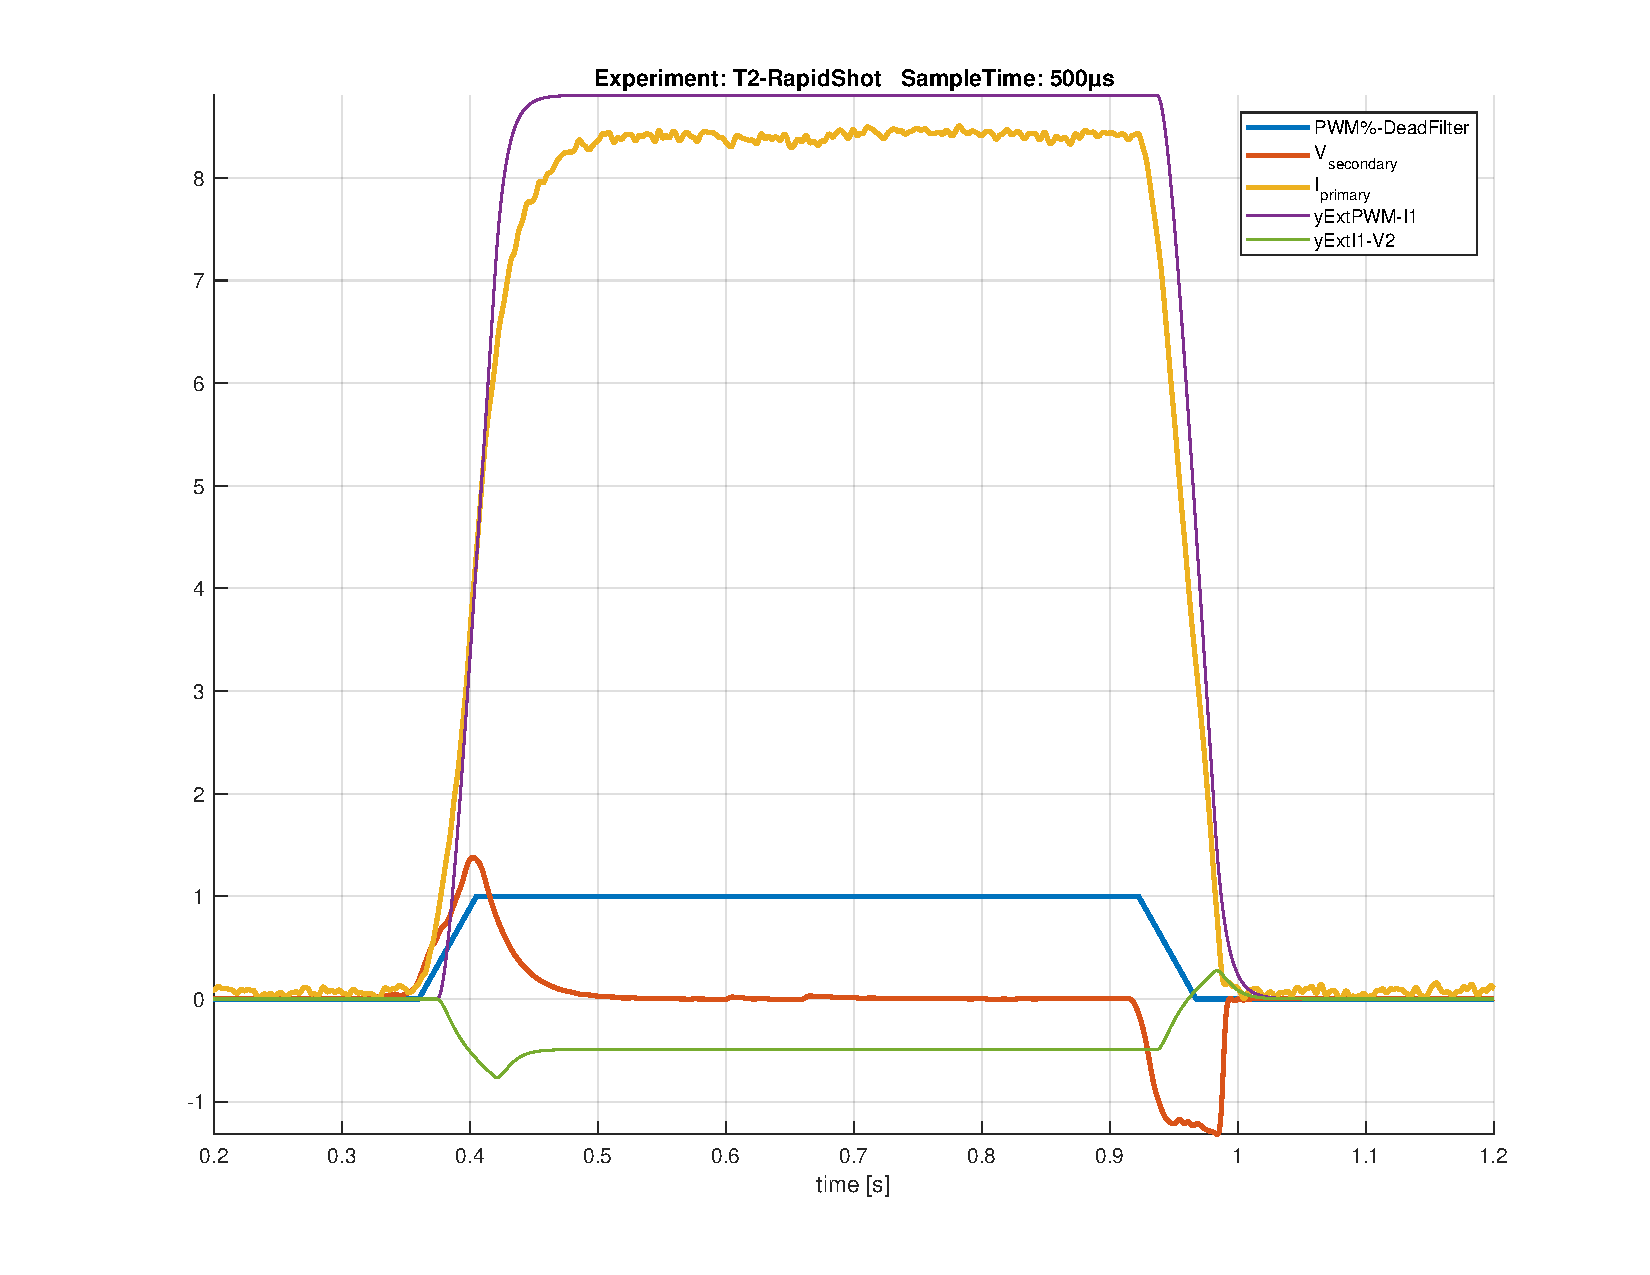
\includegraphics[width=1\textwidth]{Stime/T2-RapidShot-autoExt.pdf}
\end{figure}

\noindent
Analizzando il grafico abbiamo che i primi 3 segnali (spessi), sono i dati reali dell'esperimento filtrati (\nameref{subsec:filtraggio}), mentre le altre 2 linee rappresentano la simulazione usando la stima del Toolbox come modello.\\
Risulta facile vedere che la corrente del primario è accettabile anche se migliorabile, ma la funzione di trasferimento stimata per il secondario è completamente sbagliata, anche se dimensionalmente è simile.\\
Usando queste stime come base si sono trovati a mano dei coefficienti che meglio approssimano l'andamento delle curve.


\section{Tuning dei coefficienti}
Partendo dai modelli generati da \cite*{IdentificationToolbox} e riportati in tabella \ref{tab:stimaAutomaticaParametri}, si sono "\textit{limati}" i dati a mano" per migliorare la stima dei parametri, di seguito è riportata la tabella con i valori migliorati:
\begin{table}[H]
	\centering
	\caption[Stime parametri tarati a mano]{Stime parametri tarati a mano}		\label{tab:stimaManualeParametri}
	\vspace{1mm}
	\begin{tabular}[t]{||l|c|c||}
		\hline
		\multicolumn{1}{||c}{\textbf{Funzione}}                                                & \multicolumn{1}{|c}{\textbf{Input}} & \multicolumn{1}{|c||}{\textbf{Input}} \\
		\hline\hline
		                                                                                       &                                     &                                       \\[-3mm]
		$\tilde{P}_{p_{wm} I_1}(s) = \frac{8.4}{0.022\,s+1}$                                   & PWM                                 & $I_1$                                 \\[3mm]

		$\tilde{P}_{I_1 V_2}(s) = \frac{\num{8.5e-3}\,s}{\num{3.6e-4}\,s+1}$                   & $I_1$                               & $V_2$                                 \\[3mm]

		$\tilde{P}_{p_{wm} V_2}(s) = \frac{\num{9.1e+3}\,s}{s^2+\num{2.8e+3}\,s+\num{1.3e+5}}$ & PWM                                 & $ V_2 $                               \\
		\hline
	\end{tabular}
\end{table}

\begin{figure}[H]
	\centering
	\caption[Simulazione con parametri tarati a mano]{Simulazione con parametri tarati a mano}
	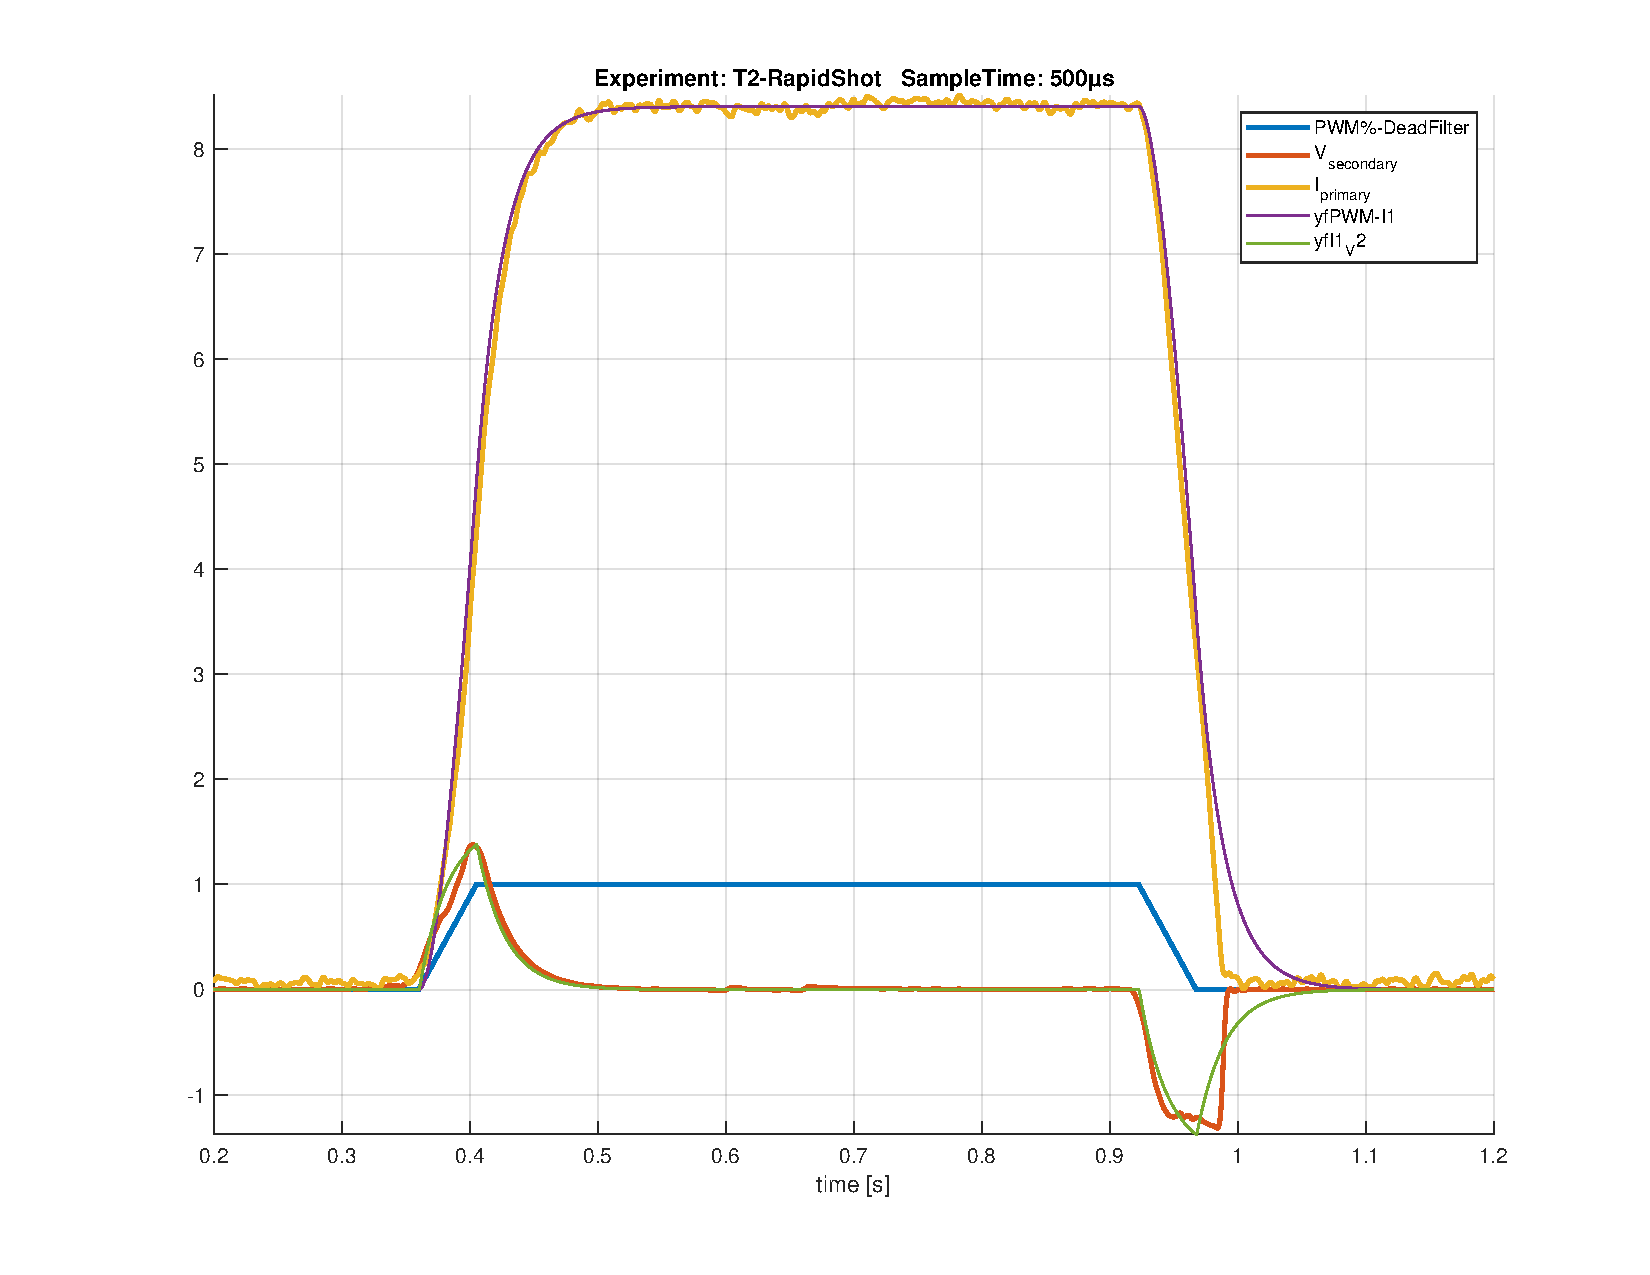
\includegraphics[width=1\textwidth]{Stime/T2-RapidShot-manualExt.pdf}
\end{figure}
\noindent
In particolare nella Dead-Zone inferiore il modello non risulta accurato, essendo predominanti le dinamiche non lineari, e ciò si vede particolarmente bene sul fronte di discesa del sistema, ma nel complesso la funzione trovata è una buona candidata per uno studio teorico e simulativo del sistema prima di passare alla fase implementativa reale.

\section{Benchmark}

In questa sezione alcune frazioni interessanti di un esperimento lungo con vari segnali e metteremo a confronto il modello trovato con i risultati reali.
\begin{figure}[H]
	\centering
	\caption[Esperimento di verifica della stima 1]{Esperimento di verifica della stima 1}
	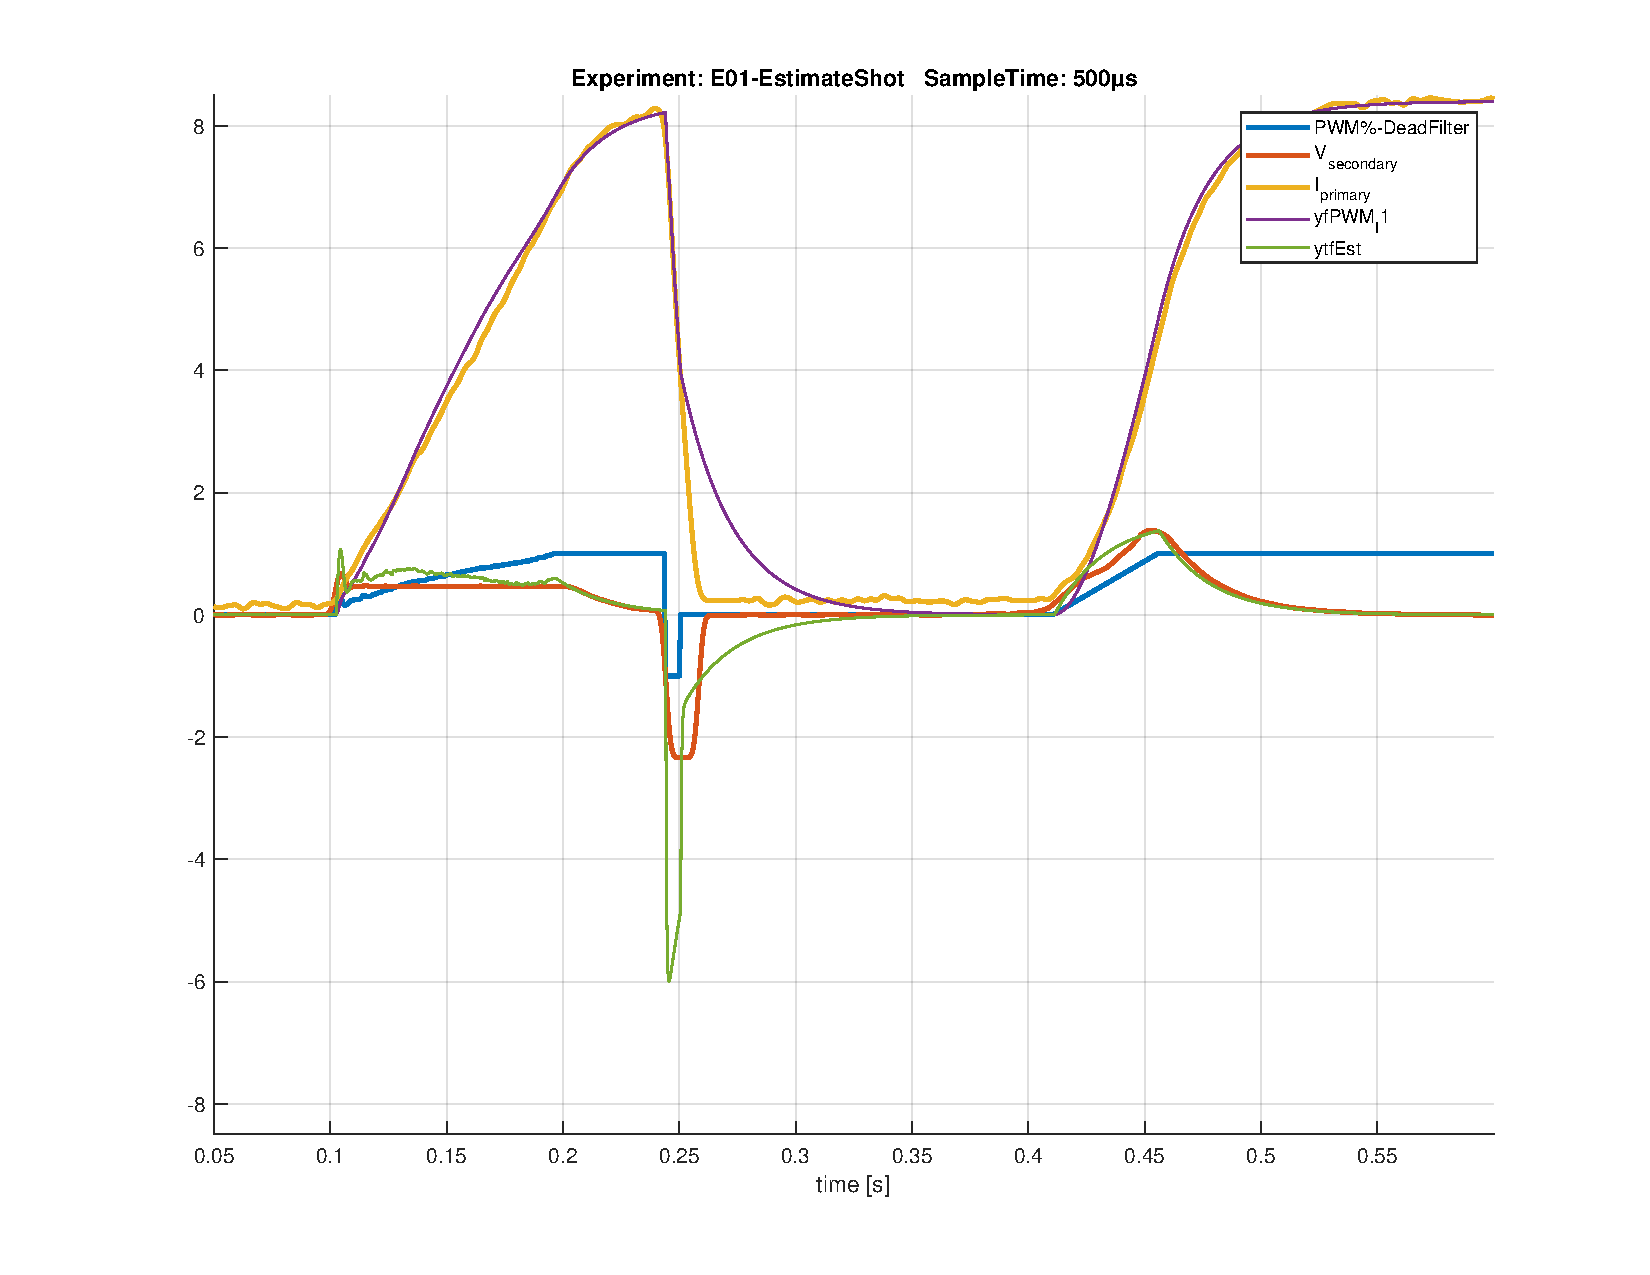
\includegraphics[width=0.8\textwidth]{Stime/E01-EstimateShot-manual-1.pdf}
\end{figure}

\begin{figure}[H]
	\centering
	\caption[Esperimento di verifica della stima 2]{Esperimento di verifica della stima 2}
	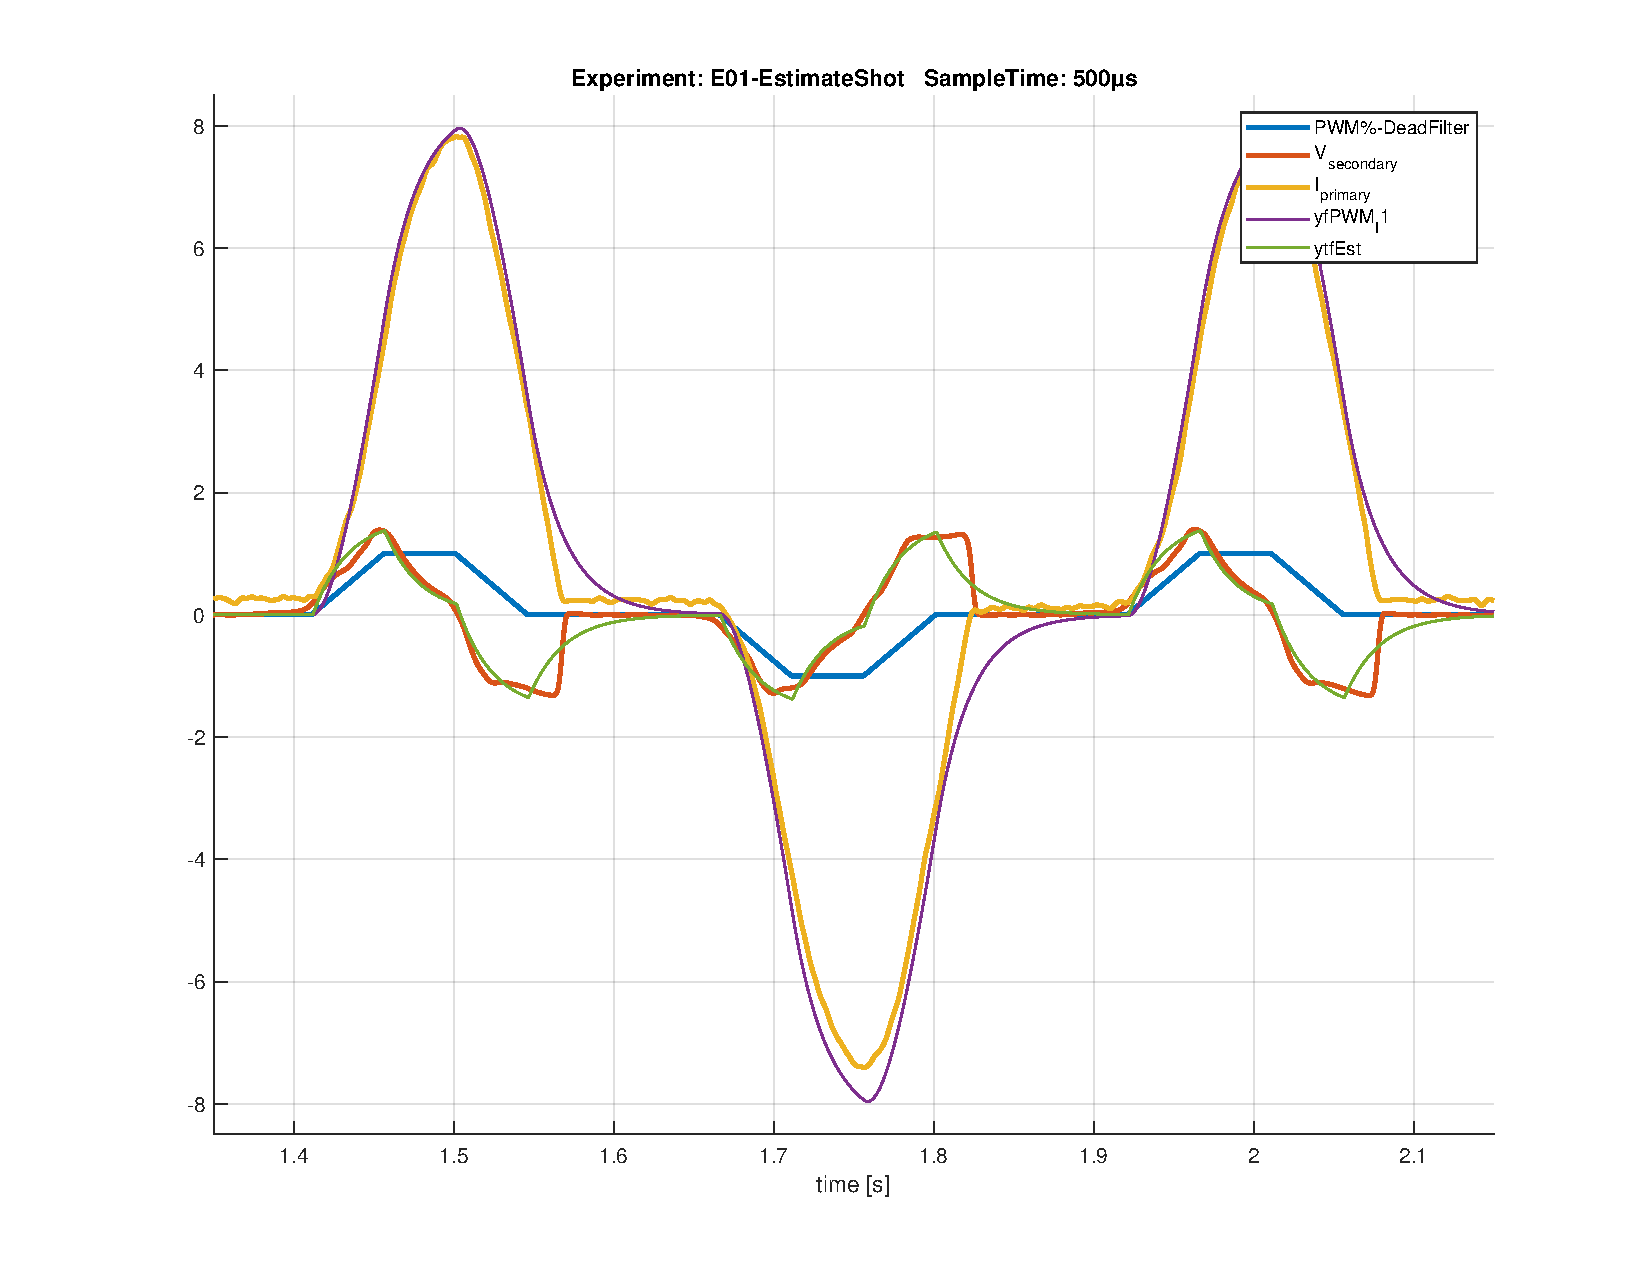
\includegraphics[width=0.8\textwidth]{Stime/E01-EstimateShot-manual-2.pdf}
\end{figure}

\begin{figure}[H]
	\centering
	\caption[Esperimento di verifica della stima 3]{Esperimento di verifica della stima 3}
	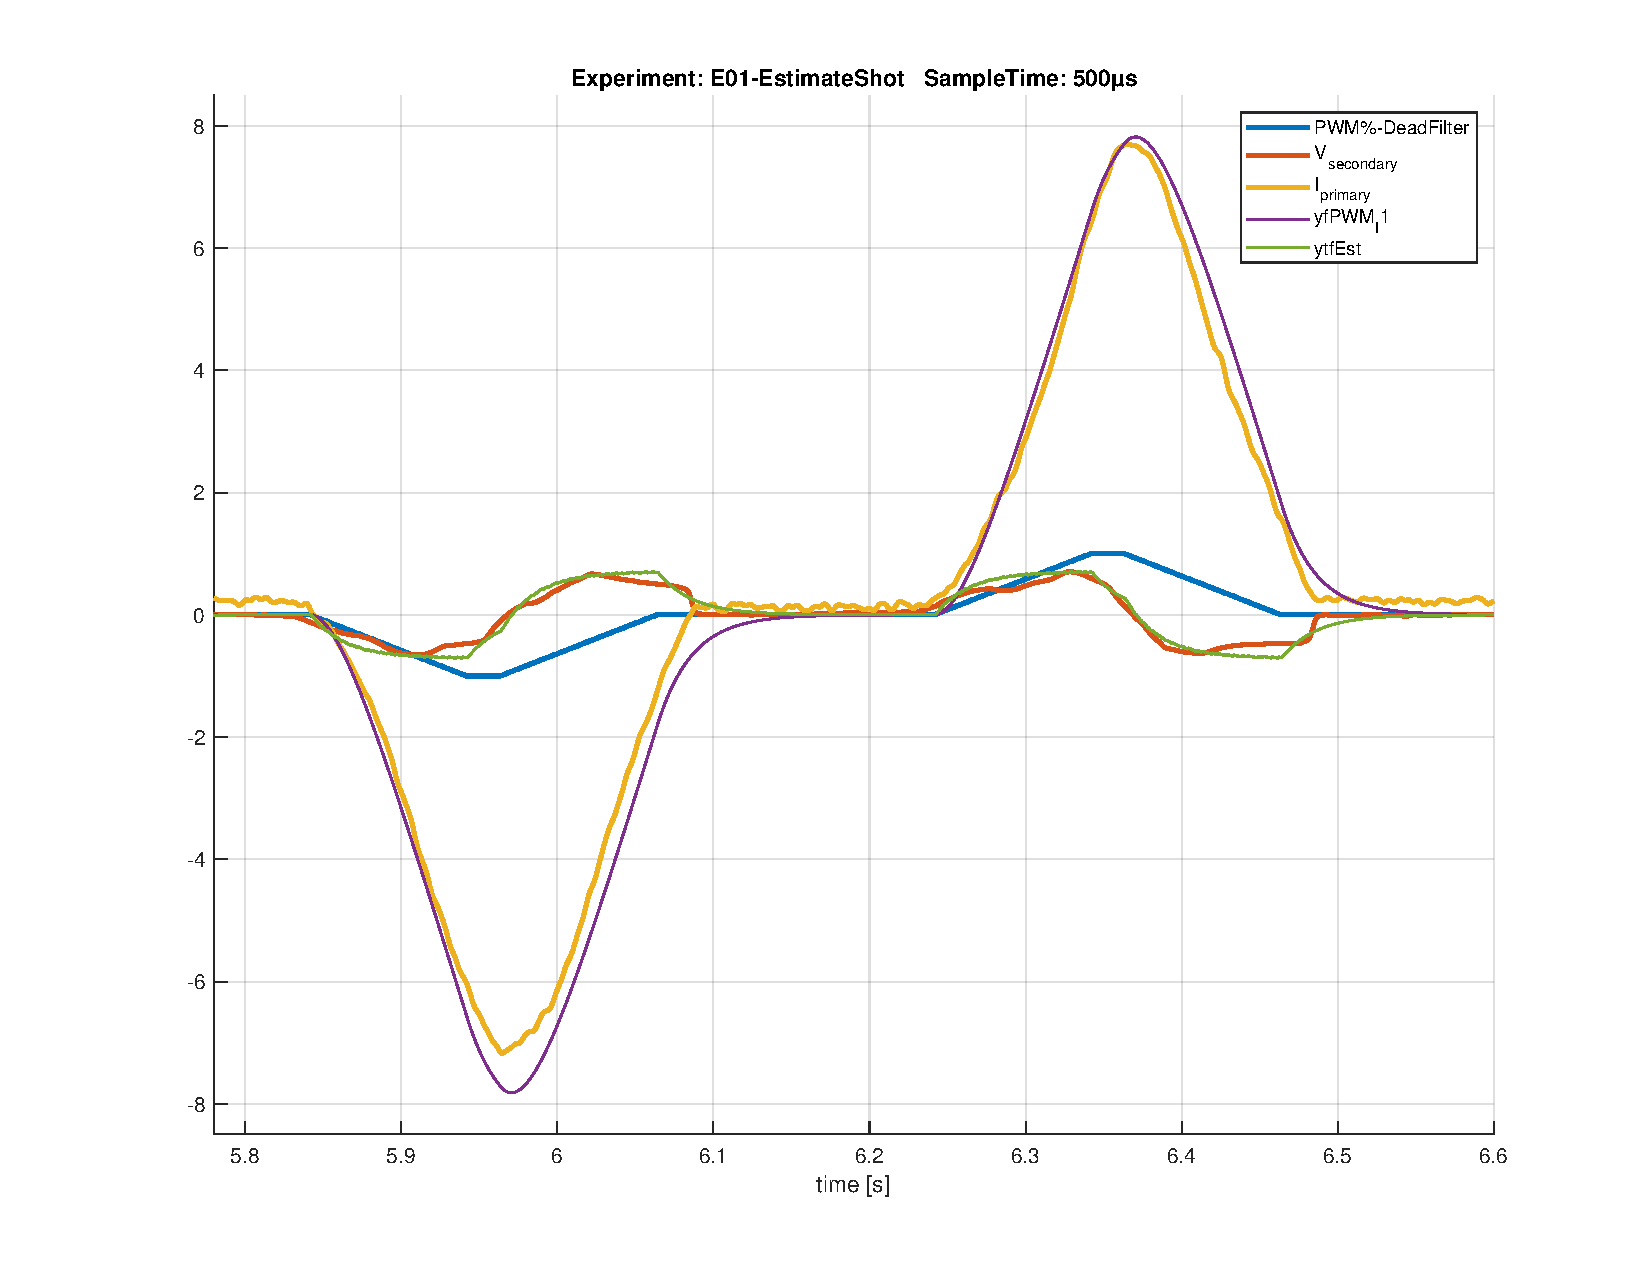
\includegraphics[width=0.8\textwidth]{Stime/E01-EstimateShot-manual-3.pdf}
\end{figure}

Da questi grafici risulta chiaro che, anche se non perfetto, e certamente trascurando delle \nonLinearita del sistema originale, la dinamica simulata è rappresentativa dell'andamento reale del sistema complessivo.
La funzione di trasferimento :
\begin{empheq}[box=\mathResult]{equation}	\label{eq:StimaModelloInOut}
\tilde{P}_{p_{wm} V_2}(s) = \frac{\num{9.1e+3}\,s}{s^2+\num{2.8e+3}\,s+\num{1.3e+5}}
\end{empheq}
verrà da ora considerata la funzione stimata del modello e usata nelle simulazioni.




